\documentclass[a4paper, 10pt]{article}

\usepackage{vmargin}

\setmarginsrb{2cm}{0cm}{2cm}{0,2cm}{1cm}{1,5cm}{1cm}{1,5cm}
%1 est la marge gauche
%2 est la marge en haut
%3 est la marge droite
%4 est la marge en bas
%5 fixe la hauteur de l'entête
%6 fixe la distance entre l'entête et le texte
%7 fixe la hauteur du pied de page
%8 fixe la distance entre le texte et le pied de page
%------------------------------Packages généraux------------------------------

\usepackage[english]{babel}
\usepackage[T1]{fontenc}
\usepackage{ae}
\usepackage[utf8]{inputenc}
\usepackage{scrextend}
\usepackage{hyperref}

%-------------------------Mathématiques------------------------------
\usepackage{amsmath}
\usepackage{amssymb}
\usepackage{amsthm}
\usepackage{amsfonts}
\usepackage{eucal}
\newcommand\independent{\protect\mathpalette{\protect\independenT}{\perp}}
\def\independenT#1#2{\mathrel{\rlap{$#1#2$}\mkern2mu{#1#2}}}
%-----------------------Codes et algorithmes--------------------------
\usepackage{algorithm}
\usepackage{algorithmic}
\usepackage{clrscode3e}

%------------------------------Graphics------------------------------

\usepackage{graphicx}
\usepackage{fancyhdr}
\usepackage{fancybox}
\usepackage{color}
\usepackage{pgf, tikz}
\usetikzlibrary{arrows, automata}
%\usepackage{slashbox}
%------------------------------Syntaxe------------------------------

\usepackage{listings}
\lstloadlanguages{Matlab}

\def\refmark#1{\hbox{$^{\ref{#1}}$}}
\DeclareSymbolFont{cmmathcal}{OMS}{cmsy}{m}{n} %Mathcal correcte
\DeclareSymbolFontAlphabet{\mathcal}{cmmathcal}

%------------------------------Inclure code MatLab------------------------------

\usepackage{listings}
\newcommand*\styleC{\fontsize{9}{10pt}\usefont{T1}{ptm}{m}{n}\selectfont }
\newcommand*\styleD{\fontsize{9}{10pt}\usefont{OT1}{pag}{m}{n}\selectfont }

%------------------Sub-sections--------%
\usepackage{titlesec}
\usepackage{hyperref}

\renewcommand\thesubsubsection{\alph{subsubsection}}

\titleclass{\subsubsubsection}{straight}[\subsubsection]

\newcounter{subsubsubsection}[subsubsection]
\renewcommand\thesubsubsubsection{\thesubsubsection.\arabic{subsubsubsection}}

\titleformat{\subsubsubsection}
  {\normalfont\normalsize\bfseries}{\thesubsubsubsection}{1em}{}
\titlespacing*{\subsubsubsection}
{0pt}{3.25ex plus 1ex minus .2ex}{1.5ex plus .2ex}


\makeatletter
% on fixe le langage utilisé
\lstset{language=matlab}
\edef\Motscle{emph={\lst@keywords}}
\expandafter\lstset\expandafter{%
  \Motscle}
\makeatother


\definecolor{Ggris}{rgb}{0.45,0.48,0.45}

\lstset{emphstyle=\rmfamily\color{blue}, % les mots réservés de matlab en bleu
basicstyle=\styleC,
keywordstyle=\ttfamily,
commentstyle=\color{Ggris}\styleD, % commentaire en gris
numberstyle=\tiny\color{red},
numbers=left,
numbersep=10pt,
lineskip=0.7pt,
showstringspaces=false}
%  % inclure le fichier source
\newcommand{\FSource}[1]{%
\lstinputlisting[texcl=true]{#1}
}

\usepackage[section]{placeins}

\let\cleardoublepage\clearpage

\usepackage{hyperref}
               
 \hypersetup{
    colorlinks = true,
    linkcolor=black,
    urlcolor = black
    }
%------------------------------Début du document------------------------------
\begin{document}
%------------------------------Page de garde------------------------------

  % \frontmatter
  %\tableofcontents
   \newpage
   \setcounter{page}{1}
   %%%%%%%%% TP 1 %%%%%%%%%%%
   \section{Solving problems by searching (11/10/2018)}
   \subsection{Objectives}
   At the end of this exercise session you should be able to:
   \begin{itemize}
       \item Define rigorously what is a "Search Problem".
       \item Theoretically (COST\footnote{Completeness-Optimality-Space Complexity-Time Complexity}) analyse the algorithms to do uninformed (Depth-first, Breadth-first, Uniform-cost) and informed (Greedy-search, A-star) search.
       \item Be able to apply each of these algorithms on any search problem define in a fully observable and deterministic environment.
   \end{itemize}
   \subsection{Exercises}
   \subsubsection{Search algorithms ($\approx$ 35 min)}
   \begin{tikzpicture}[
            -> = stealth, % arrow head style
            %shorten > = 1pt, % don't touch arrow head to node
            auto,
            node distance = 3cm, % distance between nodes
            semithick % line style
        ]

        \tikzstyle{every state}=[
            draw = black,
            thick,
            fill = white,
            minimum size = 12mm
        ]

        \node[state, align=center] (S) {Start};
        \node[state, align=center] (A) [above right of=S] {A\\h=20};
        \node[state, align=center] (B) [right of=S] {B\\h=12};
        \node[state, align=center] (C) [below right of=S] {C\\h=10};
        \node[state, align=center] (D) [below right of=B] {D\\h=25};
        \node[state, align=center] (E) [above right of=B] {E\\h=19};
        \node[state, align=center] (F) [right of=D] {Goal};

        \path[-] (S) edge node {1} (A);
        \path[-] (S) edge node {4} (B);
        \path[-] (S) edge node {3} (C);
        \path[-] (B) edge node {5} (D);
        \path[-] (B) edge node {5} (E);
        \path[-] (D) edge node {10} (F);
        \path[-] (E) edge node {20} (F);
        \path[-] (C) edge node {2} (B);
        \path[-] (A) edge node {5} (B);

        %\draw[red, dashed] (1, 2) -- (1, -2);
    \end{tikzpicture}
    \\
    For each of the following search algorithms, give the order in which states are expanded as well as the final path returned by the algorithm. If two nodes are in competition to be expanded, the conflict is resolved by alphabetical order.
    \begin{enumerate}
        \item Depth-First
        \item Breadth-First
        \item Uniform-Cost
        \item Greedy
        \item A-Star (Is the heuristic admissible?)
    \end{enumerate}
   \subsubsection{Maze Car ($\approx$ 25 min)}
   %The project RAGI aims at building an agent,	
%meant	to	recognize	people	entering	a	building, welcome	them	and	guide	them	into Montefiore Institute,	
%in	a	smart	way. 
   %Imagine a car-like agent wishes to guide a visitor to Professor Louppe's office a maze like the one shown below:
Imagine a car-like agent wishes to exit a maze like the one shown below:
\\
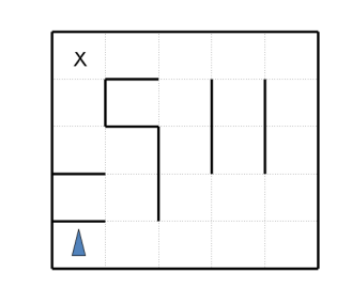
\includegraphics[scale=1]{figures/tp1_maze.png}\\
The agent is directional and at all times faces some direction d $\in$ (N, S, E, W). With a single action, the agent
can either move forward at an adjustable velocity v or turn. The turning actions are left and right, which change
the agent’s direction by 90 degrees. Turning is only permitted when the velocity is zero (and leaves it at zero).
The moving actions are fast and slow. Fast increments the velocity by 1 and slow decrements the velocity by 1;
in both cases the agent then moves a number of squares equal to its NEW adjusted velocity. Any action that
would result in a collision with a wall crashes the agent and is illegal. Any action that would reduce v below 0
or above a maximum speed $V_{max}$ is also illegal. The agent’s goal is to find a plan which parks it (stationary)
on the exit square using as few actions (time steps) as possible.
As an example: if the agent shown were initially stationary, it might first turn to the east using (right), then
move one square east using fast, then two more squares east using fast again. The agent will of course have to
slow to turn.
\begin{itemize}
    \item Quizz ($\approx 15$ minutes):
    \begin{enumerate}
    \item If the grid is M by N, what is the size of the state space? You should assume that all configurations are reachable from the start state. 
    \item What is the maximum branching factor of this problem? You may assume that illegal actions are simply not returned by the successor function.
    \item Is the Manhattan distance from the agent’s location to the exit’s location admissible?
    \item If we used an inadmissible heuristic in A* tree search, could it change the completeness of the search?
    \item If we used an inadmissible heuristic in A* tree search, could it change the optimality of the search?
    \end{enumerate}
    \item Discussion (if time permits) ($\approx 10$ minutes):
    \begin{enumerate}
        \item State and justify a non-trivial admissible heuristic for this problem.
        \item Give a general advantage that an inadmissible heuristic might have over an admissible one.
    \end{enumerate}
\end{itemize}
   \subsection{Supplementary material}
   \url{http://ai.berkeley.edu/sections/section_0_v55LOfoUUwiW1k6Nchnk3Dw6WQuTW8.pdf}\\
   \url{http://ai.berkeley.edu/sections/section_1_0hzy6TFupb1Z3bckfRXdC5KYpsdZOE.pdf}\\
\end{document}
